%% Solutions to part 2
\pagebreak

\subsubsection*{2.A}


\subsubsection*{2.B}
The Matlab code to calculate the learning curve is included below. Figure~\ref{fig:part2-learning-curve} shows the learning curve averaged over 100 independent input realizations, and  Figure~\ref{fig:part2-weights} shows the converged weight vector. 

Note that the learning curve converged to a much smaller MMSE. Note further that the bias weight is practically negligible now, and some of the weights corresponding to the squared inputs and to the cross-products are significant. 

\FloatBarrier
\begin{figure}[h!]
	\centering
	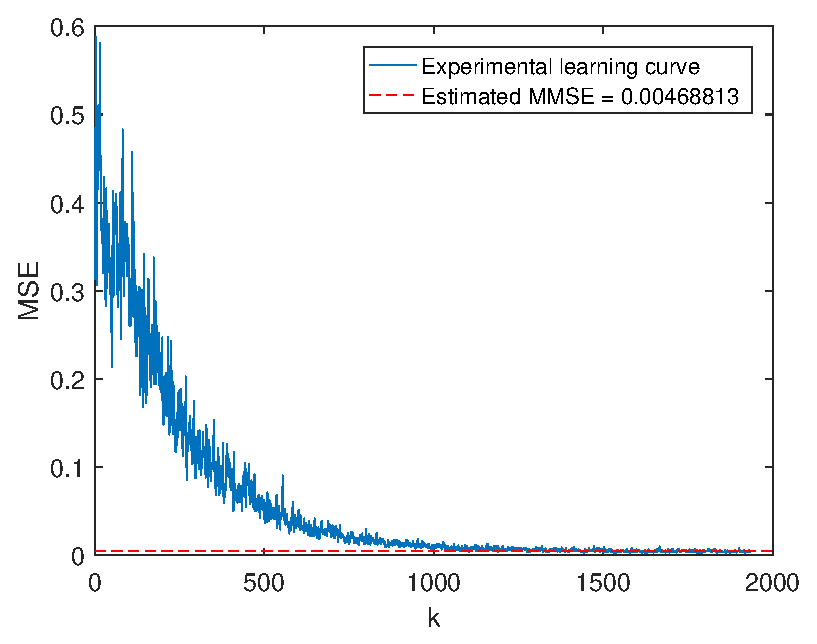
\includegraphics[scale=0.8]{part2_learning_curve.eps}
	\caption{Experimental learning curve for nonlinear plant identification using a nonlinear filter based on Volterra series. The learning curve was averaged 100 times. The training signal had variance $\sigma_r^2 = 4$.}
	\label{fig:part2-learning-curve}
\end{figure}
\FloatBarrier

\FloatBarrier
\begin{figure}[h!]
	\centering
	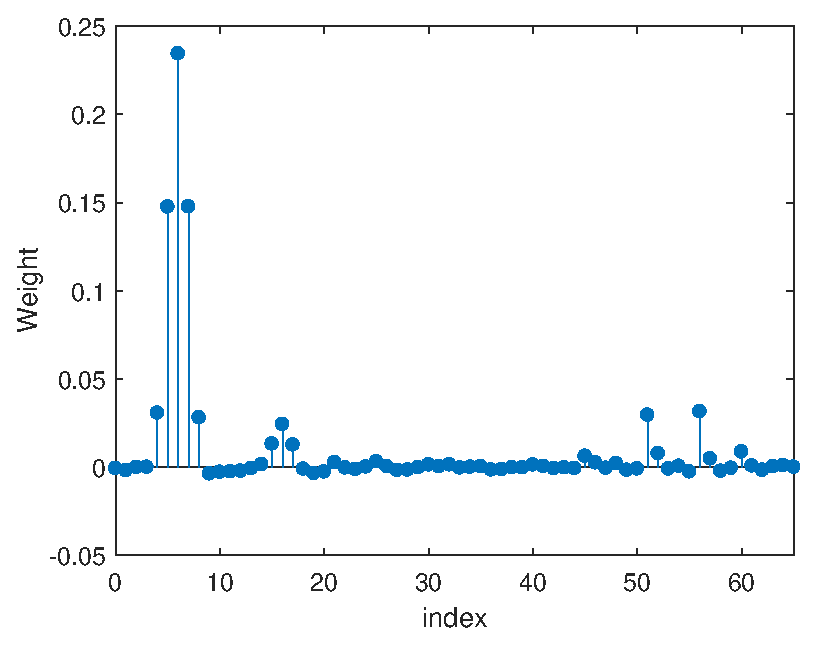
\includegraphics[scale=0.8]{part2_weights.eps}
	\caption{Weight vector after convergence.}
	\label{fig:part2-weights}
\end{figure}
\FloatBarrier

\subsubsection*{2.C}

As shown in Figure~\ref{fig:part2-learning-curve}, the MMSE estimated using the last 200 samples was equal to $\approx 0.0046$.

\subsubsection*{2.D}
The Matlab code is included in the appendix. The output of the plant is compared to the output of the adaptive filter in Figure~\ref{fig:part2-test}. 

The adaptive filter was trained with random signal, but it can almost perfectly track the plant output to a sinusoidal input. The same cannot be accomplished when the adaptive filter is linear as in part 1.E.

\FloatBarrier
\begin{figure}[h!]
	\centering
	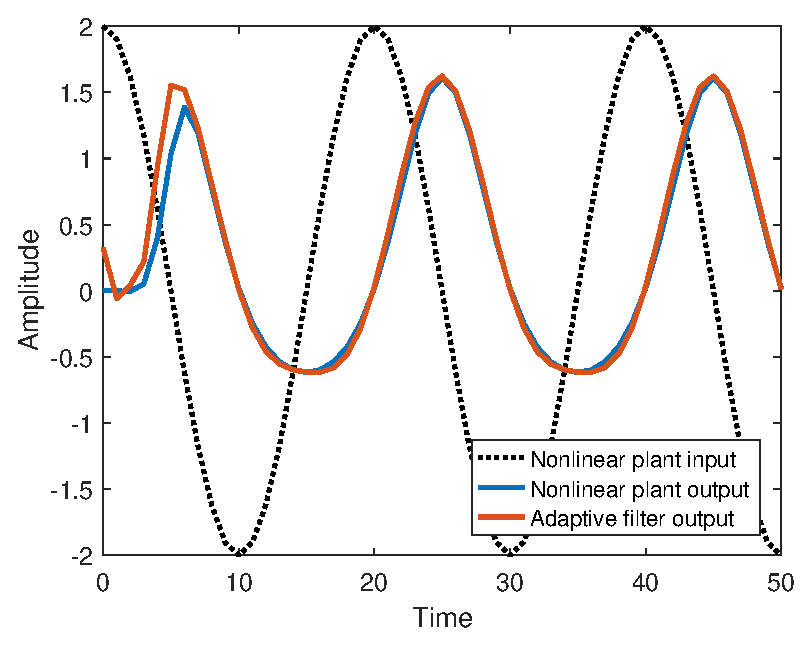
\includegraphics[scale=0.8]{part2_test.eps}
	\caption{Test of the adaptive filter after convergence with a sinusoidal signal. During the first $L+1$ samples, the filter was being initialized.}
	\label{fig:part2-test}
\end{figure}
\FloatBarrier

\subsubsection*{2.E}

When the training signal variance was $\sigma_r^2 = 0.4$, the adaptive filter achieved MMSE equal to $1.8\times 10^{-5}$ during training, but it didn't performed as well as before during test with a sinusoidal signal. The reason for this is that for a smaller training signals, the plant is approximately linear, and the adaptive equalizer cannot learn well the weights that weigh the nonlinear terms of the input. 

\FloatBarrier
\begin{figure}[h!]
	\centering
	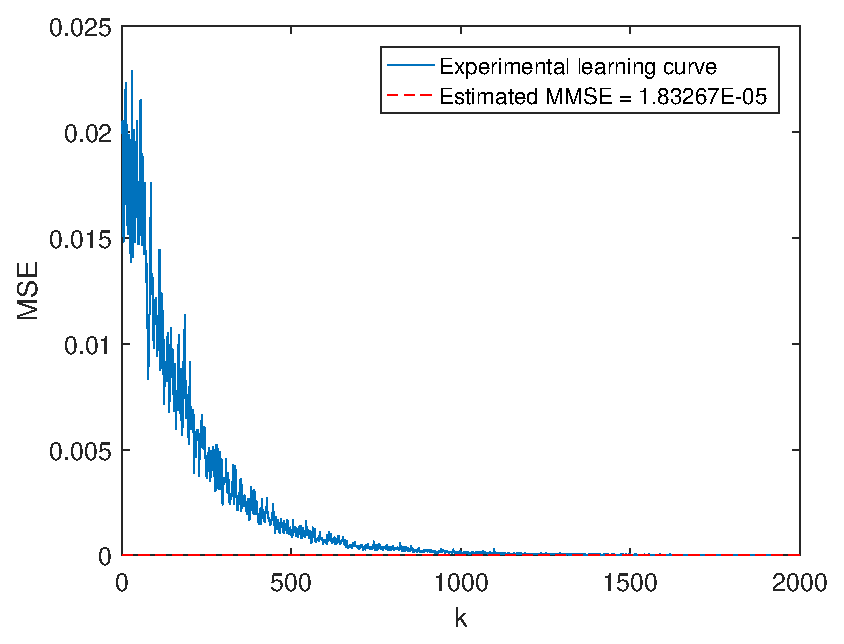
\includegraphics[scale=0.8]{part2e_learning_curve.eps}
	\caption{Experimental learning curve for nonlinear plant identification using a nonlinear filter based on Volterra series. The learning curve was averaged 100 times. The training signal had variance $\sigma_r^2 = 0.4$.}
	\label{fig:part2e-learning-curve}
\end{figure}
\FloatBarrier

\FloatBarrier
\begin{figure}[h!]
	\centering
	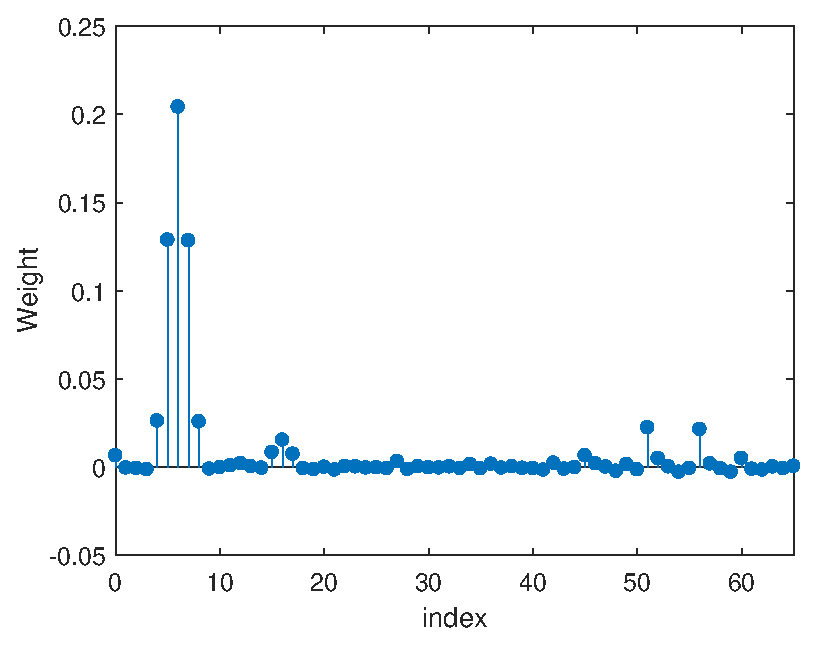
\includegraphics[scale=0.8]{part2e_weights.eps}
	\caption{Weight vector after convergence.}
	\label{fig:part2e-weights}
\end{figure}
\FloatBarrier

\FloatBarrier
\begin{figure}[t!]
	\centering
	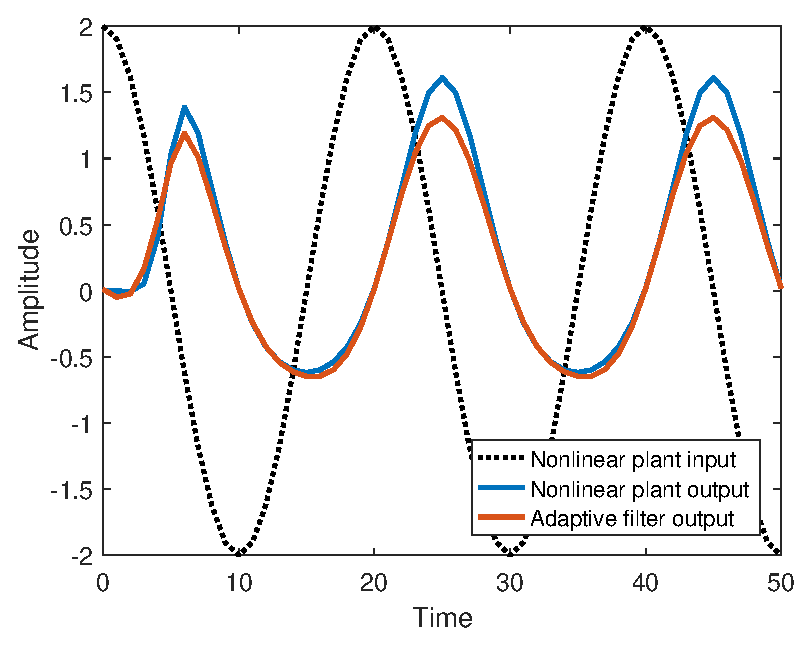
\includegraphics[scale=0.8]{part2e_test.eps}
	\caption{Test of the adaptive filter after convergence with a sinusoidal signal. During the first $L+1$ samples, the filter was being initialized.}
	\label{fig:part2e-test}
\end{figure}
\FloatBarrier
